\scanpage{71}
\mspage{\deleted{\unsure{69|79}}\unsure{70|79}}

Il revient au $=$ de dire que $F$ et $F'$ ont $=$ cosupport, ou encore, même support.

\unsure{Donnons nous} un support.

% R2-margin-marks: the two disconnected groups are drawn, without assigning them a linguistic function.
\figure{
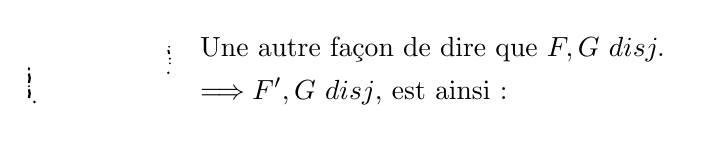
\begin{tikzpicture}[x=1cm,y=1cm]
  \node[anchor=north west,align=left] at (2.15,0.55) {Une autre façon de dire que $F,G\ \text{disj.}$\\[0.35em]
  $\Longrightarrow F',G\ \text{disj}$, est ainsi :};
  \fill (0.10,0.02) ellipse (0.016 and 0.024);
  \draw[line width=0.8pt] (0.10,-0.04)--(0.11,-0.10)--(0.10,-0.16);
  \fill (0.10,-0.20) circle (0.014);
  \draw[line width=0.8pt] (0.10,-0.24)--(0.11,-0.29)--(0.10,-0.35);
  \fill (0.17,-0.40) circle (0.018);
  \fill (1.88,0.30) circle (0.013);
  \draw[line width=0.7pt] (1.87,0.26)--(1.88,0.21);
  \fill (1.89,0.15) circle (0.015);
  \fill (1.89,0.09) circle (0.013);
  \fill (1.87,-0.03) circle (0.017);
\end{tikzpicture}}

% R2-corollary-correction: de is crossed by the long rising stroke under the raised addition.
\figure{
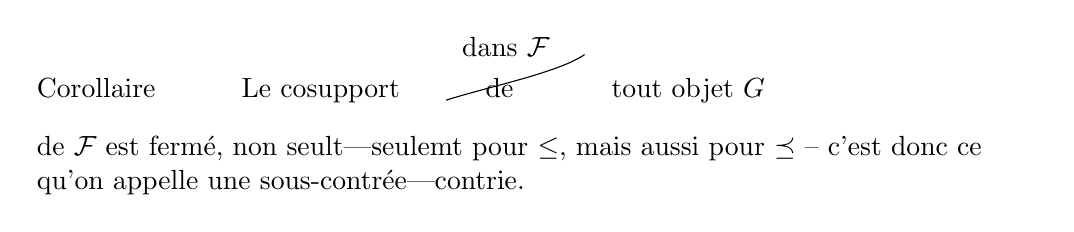
\begin{tikzpicture}[x=1cm,y=1cm]
  \node[anchor=base west] at (0,0) {\uline{Corollaire}};
  \node[anchor=base west] at (2.60,0) {Le cosupport};
  \node[anchor=base west] at (5.70,0) {\deleted{de}};
  \node[anchor=base west] at (5.40,0.52) {\inserted{dans $\mathcal F$}};
  \draw (5.32,-0.04) .. controls (5.85,0.13) and (6.75,0.31) .. (7.08,0.54);
  \node[anchor=base west] at (7.30,0) {tout objet $G$};
  \node[anchor=north west,text width=12.7cm,align=left] at (0,-0.38) {de $\mathcal F$ est fermé, non \unsure{seult|seulemt} pour $\leq$, mais aussi pour $\preceq$ -- c'est donc ce qu'on appelle une \uline{sous}-\unsure{contrée|contrie}.};
\end{tikzpicture}}

% R2-itou-mark: the final detached high stroke is reproduced; its role in the word is uncertain.
\figure{

\begin{tikzpicture}[x=1cm,y=1cm]
  \node[anchor=base west] at (0,0) {Donc};
  \node[anchor=base west] at (1.15,0) {\unsure{itou|itout}};
  \draw (1.91,0.33)--(1.96,0.49)--(2.03,0.38);
  \node[anchor=base west] at (3.45,0) {pour toute partie $\Phi\subset\mathcal F$.};
\end{tikzpicture}}

% R2-right-punctuation: the punctuation after leq is drawn in place. The loop and short right arm meet the sheet edge.
\figure{
\begin{tikzpicture}[x=1cm,y=1cm]
  \node[anchor=base west] at (0,0) {En d'autres termes, \deleted{toute} partie};
  \node[anchor=base west] at (0,-0.58) {de $\mathcal F$ qui est un $\mathcal F$-support (ou};
  \node[anchor=base west] at (0,-1.16) {``$\mathcal F$-\unsure{saturee|saturée}, sous-entendu : en termes de $\leq$};
  \node[anchor=base west] at (12.05,-1.16) {\unsure{\begin{tikzpicture}[x=1cm,y=1cm,baseline=0pt]
    \draw[line width=0.6pt] (0.04,0.01) .. controls (0.09,-0.09) and (0.04,-0.17) .. (-0.02,-0.20);
    \draw (0.16,0.36) .. controls (0.43,0.10) and (0.43,-0.10) .. (0.23,-0.23);
    \draw (0.30,0.22) .. controls (0.33,0.26) and (0.38,0.18) .. (0.45,0.17) .. controls (0.54,0.15) and (0.41,0.08) .. (0.35,0.04);
    \draw (0.37,0.02)--(0.54,-0.02);
  \end{tikzpicture}}};
  \node[anchor=base west] at (0,-1.85) {cf page $67$) est \unsure{automatiquemt|automatiquement} \deleted{\unsure{f}}une};
  \node[anchor=base west] at (0,-2.43) {sous-contrée.};
\end{tikzpicture}}

% Cancelled draft, written upside down. Its folio belongs to the cancelled draft.
\mspage{\deleted{5\deleted{\unsure{4|3}}5}}
% R2-cancelled-draft: all text occurs once in the rotated nodes; the enclosure and long cancellation strokes are drawn separately.
\figure{
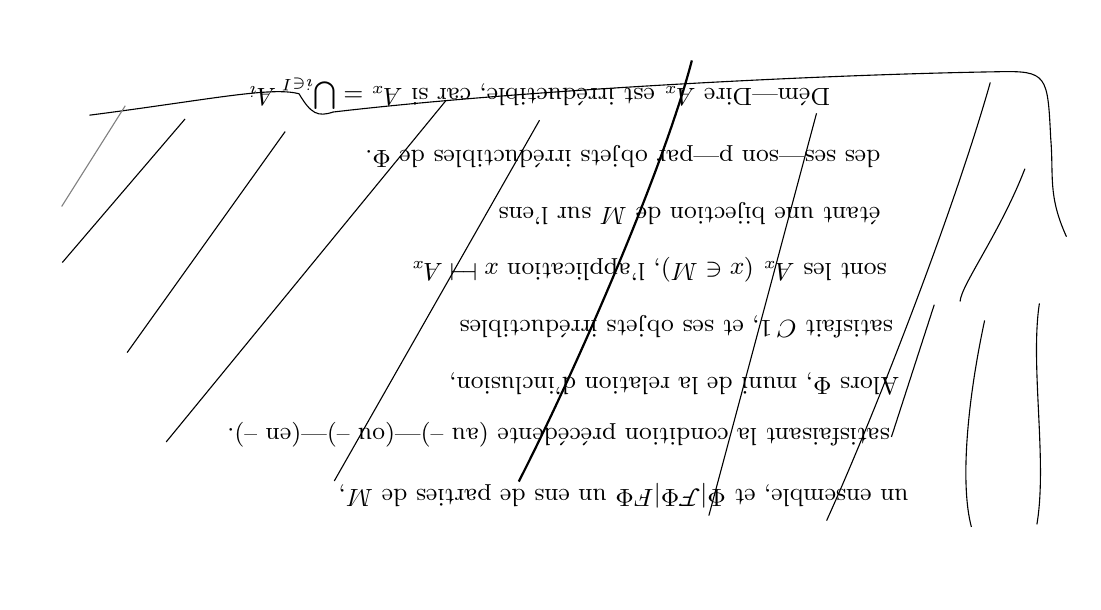
\begin{tikzpicture}[x=0.008cm,y=-0.008cm]
  \path[use as bounding box] (20,1465) rectangle (1680,2345);
  \node[anchor=west,rotate=180,font=\small] at (1435,2208) {\deleted{un ensemble, et $\unsure{\Phi|\deleted{\mathcal F}\Phi|\deleted{F}\Phi}$ \unsure{un} ens de parties de $M$,}};
  \node[anchor=west,rotate=180,font=\small] at (1405,2112) {\deleted{satisfaisant la condition précédente \unsure{(au --)|(ou --)|(en --)}.}};
  \node[anchor=west,rotate=180,font=\small] at (1420,2030) {\deleted{Alors $\Phi$, muni de la relation d'inclusion\unsure{,}}};
  \node[anchor=west,rotate=180,font=\small] at (1410,1940) {\deleted{satisfait $C\,1$, et ses objets irréductibles}};
  \node[anchor=west,rotate=180,font=\small] at (1400,1850) {\deleted{sont les $A_x$ $(x\in M)$, l'application $x\mathrel{\vdash\joinrel\dashv}A_x$}};
  \node[anchor=west,rotate=180,font=\small] at (1390,1760) {\deleted{étant une bijection de $M$ sur l'ens}};
  \node[anchor=west,rotate=180,font=\small] at (1390,1670) {\deleted{des \deleted{\unsure{ses|son}} \deleted{\unsure{p|par}} objets irréductibles de $\Phi$.}};
  \node[anchor=west,rotate=180,font=\small] at (1310,1570) {\deleted{\unsure{Dém|Dire} $A_x$ est irréductible, car si $A_x=\bigcup_{i\in I} A_i$}};
  \draw (118,1604) .. controls (305,1580) and (407,1558) .. (451,1570)
    .. controls (470,1602) and (481,1607) .. (505,1599)
    .. controls (795,1565) and (1260,1540) .. (1560,1535)
    .. controls (1640,1533) and (1640,1540) .. (1645,1641)
    .. controls (1650,1700) and (1640,1731) .. (1670,1797);
  \draw (1627,1903) .. controls (1612,2000) and (1640,2155) .. (1623,2254);
  \draw (1540,1930) .. controls (1510,2070) and (1502,2195) .. (1519,2258);
  \draw (1604,1689) .. controls (1565,1790) and (1502,1875) .. (1501,1900);
  \draw (1549,1552) .. controls (1490,1760) and (1365,2080) .. (1289,2248);
  \draw (1460,1905)--(1392,2115);
  \draw (1273,1601)--(1102,2240);
  \draw[line width=0.8pt] (1075,1517) .. controls (1030,1690) and (890,2010) .. (800,2186);
  \draw (833,1612)--(507,2185);
  \draw (685,1580)--(240,2123);
  \draw (429,1630)--(178,1981);
  \draw (270,1610)--(75,1838);
  \draw[gray] (175,1589)--(74,1749);
\end{tikzpicture}}
